\documentclass{standalone}
\usepackage{amsmath}
\usepackage{amssymb}
\usepackage{tikz}
\usepackage{mathrsfs}
\usepackage{ifthen}

\newcommand{\perpp}{\perp\!\!\!\perp}
\DeclareMathOperator{\so}{\mathfrak{s}}
\DeclareMathOperator{\ra}{\mathfrak{r}}
\DeclareMathOperator{\supp}{supp}
\DeclareMathOperator{\id}{id}
\DeclareMathOperator{\dom}{dom}
\DeclareMathOperator{\ran}{ran}
\DeclareMathOperator{\Min}{Min}
\DeclareMathOperator{\cod}{cod}
\newcommand{\smallerthan}{<}
\newcommand{\greaterthan}{>}
\newcommand{\defeq}{:=}
\newcommand{\eqdef}{=:}

\newcommand{\cat}[1]{\textbf{#1}}
\DeclareMathOperator{\IG}{\mathscr{IG}}


\begin{document}
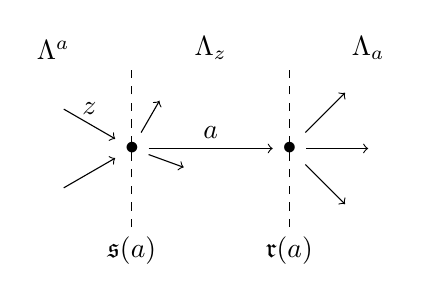
\begin{tikzpicture}
\node (Sa) at (0,0) {$\bullet$};
\node (Ra) at (2,0) {$\bullet$};
\draw[->] (Sa)--(Ra) node[above,align=center,midway] {$a$};
\draw[dashed] (Sa)+(-90:1) node[below] {$\so(a)$} -- +(90:1);
\draw[dashed] (Ra)+(-90:1) node[below] {$\ra(a)$}-- +(90:1);
\draw[->] (Sa)--+(60:0.7);
\draw[->] (Sa)--+(-20:0.7);
\node[above] at (1,1) {$\Lambda_z$};
\draw[->] (Ra) -- +(45:1);
\draw[->] (Ra) -- +(-45:1);
\draw[->] (Ra) -- +(0:1);
\draw[->] (Sa)+(150:1) -- (Sa) node[midway,above] {$z$};
\draw[->] (Sa)+(210:1) -- (Sa);
\node[above] at (3,1) {$\Lambda_a$};
\node[above] at (-1,1) {$\Lambda^a$};
\end{tikzpicture}\end{document}